\label{app:impl}

Detailing the entire implementation of the project is beyond the scope of this report. But some solutions contain non self explanatory ideas and are worthy of detailed explanations. For more details please refer to the source code.

\section{Interpolation}

One crucial detail of applying transformations to the records, is the type of interpolation used. For some images like T1 the standard trilinear interpolation makes sense, as the values inbetween voxels should be continuous. However for some other images like binary masks, the interpolation should be nearest neighbour, as the edge of the mask cant be interpreted as a fraction. And most importantly the relative connectivity and streamline images should also be interpolated with nearest neighbour, preserving their characteristics like their summed total being 1 per voxel for the relative connectivity. In theory the streamline image could be computed with trilinear interpolation, after which the relative connectivity could be computed from the interpolated streamlines. But this would degrade the streamline images due to their unbalanced nature of having a few voxels with high number of streamlines relative to the entire voxel space, effectively eroding the boundaries of the high intensity volumes.\par
In practice this meant using 0th and 1st order spline interpolations, which are numerically the same as nearest neighbour and trilinear interpolations.

\section{Multithreading}

As most of the preprocessing could not be easily offloaded to the GPU (without re-implementing major libraries such as 'pyradiomics' with GPU support), it was crucial to implement multithreading to save time.\par
The most straight forward way of doing so was to split the load on a record level, and process multiple records paralel. Testing revealed an interesting property of the feature extraction, which is the RAM IO operation bottleneck of the process. Extracting voxel based features happen in a 'voxel batch', which seemed to only increase the RAM usage of the process beyond a certain point, but not the speed. After days of tweaking and running tests, it was concluded that computing the \ac{GLCM} feature class is RAM IO operation heavy. Meaning that increasing voxel batch size or the number of threads (computing different records in parallel) will not increase the performance past a certain point, as the threads are waiting on RAM IO operations regardless.\par
The optimal settings with the used Intel Core i5-12600K CPU and 128GBs of 3200MT/s RAM, is to use 7 threads, out of which 5 are dedicated for computing the \ac{GLCM} feature class and the rest 2 are for computing other feature classes, with a voxel batch size of 1000.\par
Trying to increase performance this point by increasing the voxel batch size, or the number of threads only resulted in the same, or worse overall performance due to the computational overhead of splitting and merging the work between more threads, and using a lot more RAM.

\section{Warp Pre-Computing}
\label{app:imp-pre}

As mentioned in \reflink{sec:eval}{subsection}, computing the evaluation metrics both in native and normalized space can be done by reconstucting the spatial records from the predicted datapoints and warping them to native/normalized space, and then re-extracting the datapoints from the warped records. However this would be computationally very expensive to do so every time when calculating the evaluation metrics.\par
The solution is to pre-compute index arrays, by assigning unique indexes to the voxels of the records, warping the records, and mapping the \ac{ROI}'s flattened voxels' unique indexes between the (warped and non-warped) record pairs into an index array which can be used to quickly and efficiently convert the voxels of the \ac{ROI} between native and normalized spaces.

\begin{figure}[H]
\centering
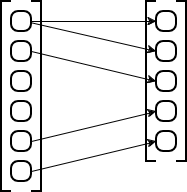
\includegraphics[width=0.3\textwidth]{warp_precompute}
\caption{Index Array Mapping}
\end{figure}

\section{Data Normalization}
\label{app:imp-norm}

As noted in \reflink{sec:norm}{subsection}, determining which voxel-based radiomic features require log scaling for distribution normalization is handled programmatically. This process involves loading each feature across all records and analyzing their distribution both before and after log scaling.\par
Initially, the feature is min-max scaled, and the distribution of non-zero voxels is calculated using $100$ bins (bin size $0.01$). Excluding zero values masks the background, which would distort the distribution. However, this exclusion should have been done with the provided brain masks, which would have been more appropriate since zeros could naturally occur in the features. This oversight, while suboptimal, does not significantly affect the results, as non-background zero counts are negligible. And the only consequence is a potential false negative artifacts (failing to apply normalization where needed), which does not degrade the raw data by inappropriately normalizing features.\par
Next, the logarithm is applied to the feature prior to min-max scaling, and the distribution is recalculated using the same $100$ bin approach. The criteria for selecting normalized features are based on observing an increased standard deviation and a reduced count of voxels in the largest bin after normalization. This ensures that features with 'flattened' and 'stretched' distributions are selected for normalization.







